% This is a sample document using the University of Minnesota, Morris, Computer Science
% Senior Seminar modification of the ACM sig-alternate style. Much of this content is taken
% directly from the ACM sample document illustrating the use of the sig-alternate class. Certain
% parts that we never use have been removed to simplify the example, and a few additional
% components have been added.

% See https://github.com/UMM-CSci/Senior_seminar_templates for more info and to make
% suggestions and corrections.

\documentclass{sig-alternate}
\usepackage{color}
\usepackage[colorinlistoftodos]{todonotes}

%%%%% Uncomment the following line and comment out the previous one
%%%%% to remove all comments
%%%%% NOTE: comments still occupy a line even if invisible;
%%%%% Don't write them as a separate paragraph
%\newcommand{\mycomment}[1]{}

\begin{document}

% --- Author Metadata here ---
%%% REMEMBER TO CHANGE THE SEMESTER AND YEAR AS NEEDED
\conferenceinfo{UMM CSci Senior Seminar Conference, December 2017}{Morris, MN}

\title{Point-of-Interest Recommendation Systems in Location-Based Social Networks}

\numberofauthors{1}

\author{
% The command \alignauthor (no curly braces needed) should
% precede each author name, affiliation/snail-mail address and
% e-mail address. Additionally, tag each line of
% affiliation/address with \affaddr, and tag the
% e-mail address with \email.
\alignauthor
Myeongjae Song\\
	\affaddr{Division of Science and Mathematics}\\
	\affaddr{University of Minnesota, Morris}\\
	\affaddr{Morris, Minnesota, USA 56267}\\
	\email{songx823@morris.umn.edu}
}

\maketitle
\begin{abstract}
The task of precise point-of-interest (POI) recommendation is a key to the success of 
location-based social networks (LBSN) since it will attract more users and advertisers 
to the platform. To achieve the POI recommendation task, many methods are proposed 
and used in practice from genetic recommendation system methods to POI specific 
algorithms. In this paper, we will analyze a novel recommendation technique named 
factorized personalized Markov chain (FPMC) model, which is a combination of matrix 
factorization and Markov chain models. We will also explore enhancements of FPMC 
optimized for POI specific characteristics such as users' movement constraint and 
complex behavior over time. Experimental results show POI specific methods outperform 
generic recommendation models. It also verifies that the more POI characteristics a system incorporates, 
the more accurate the prediction is.
\end{abstract}

\keywords{Recommendation Systems, Point-of-Interest Recommendation, Location-Based Social Networks}


\section{Introduction}
\label{sec:introduction}

Nowadays, location-based social networks (LBSN), such as \emph{Facebook places, Tinder},  and \emph{Yelp}, 
have been gaining a lot of attention with the widespread use of smartphones embedded with the 
global positioning system (GPS). Even though LBSN are relatively new compared to 
the traditional social networking services, millions of active users use the platform on a daily basis voluntarily sharing 
their location information. Many of these LBSNs allow users to ``check-in" 
places like a restaurant or cinema; we call these checked-in places the points of interest (POI) 
of the users. Users can share videos, pictures, or reviews about the places via this ``check-in" 
feature. Based on the collected user data, LBSNs provide POI recommendations. POI recommendation 
is very important for LBSNs for two reasons. First, users are more likely use the platform and check-in places 
for their own benefit if it gives accurate predictions on places where users visit next time. 
Second, it allows the advertisers launch advertisements for target user groups. Therefore, 
accurate POI recommendation is crucial for the success of LBSNs.

Even though POI recommendation is a type of recommendation system, it has distinct characteristics 
mainly due to its geographical nature. For instance, recommending a movie is a fairly different task from 
recommending a place. A movie recommendation system can recommend any movie, but a POI recommendation 
system should not just recommend a sushi restaurant in Tokyo for a user in Minnesota. The following are 
meaningful differences between conventional recommendations and POI recommendation:

\begin{figure}
\centering
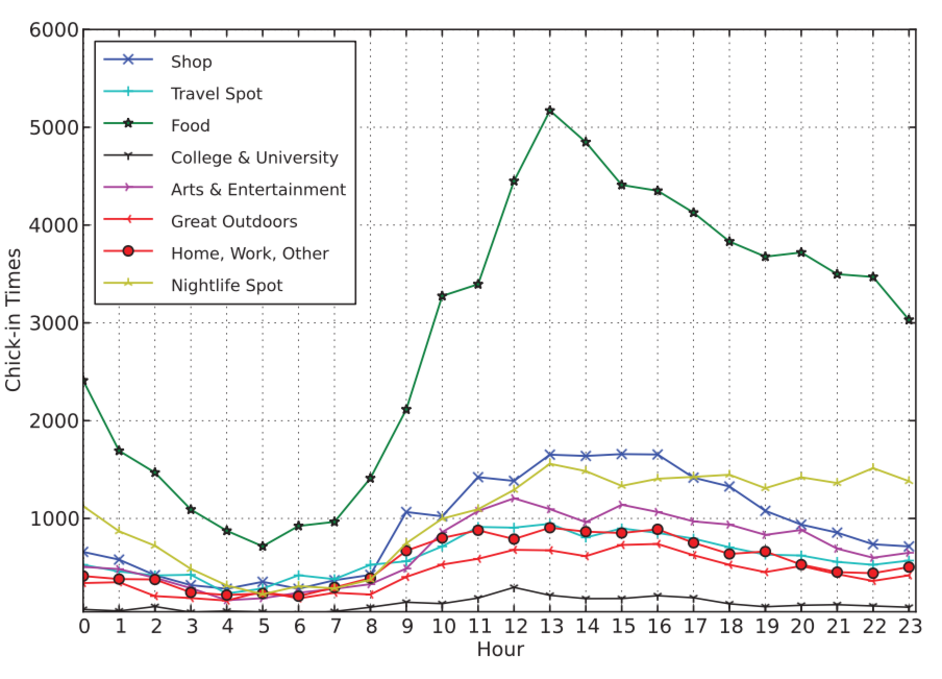
\psfig{file=NYC_checkIn.pdf,width=3.5in}
\caption{Relationship between time interval and check-in location category in NYC.}
\label{fig:NYC_checkIn}
\end{figure}

\begin{itemize}
\item[--] The types of checked-in place are highly related to the time period. Figure \ref{fig:NYC_checkIn} shows check-in data in 
NYC from a LBSN (Foursquare) over different hours of a day. The number of check-ins clearly varies depending 
on the time.
\item[--] People are likely to visit nearby places because of geographical limitation. Not many people are willing 
to fly to Japan from the US just for a nice sushi restaurant.
\item[--] The transition between POI is strongly affected by the user's own preference. Li et al. [2017] refers this as a long-term individual preference. For instance, some people go to the gym after work, but some people go home right away after work. 
\item[--] A user's next location is highly related to the user's current location. We would call this the sequential feature of POI recommendation. 
\end{itemize}

\begin{figure*}
\centering
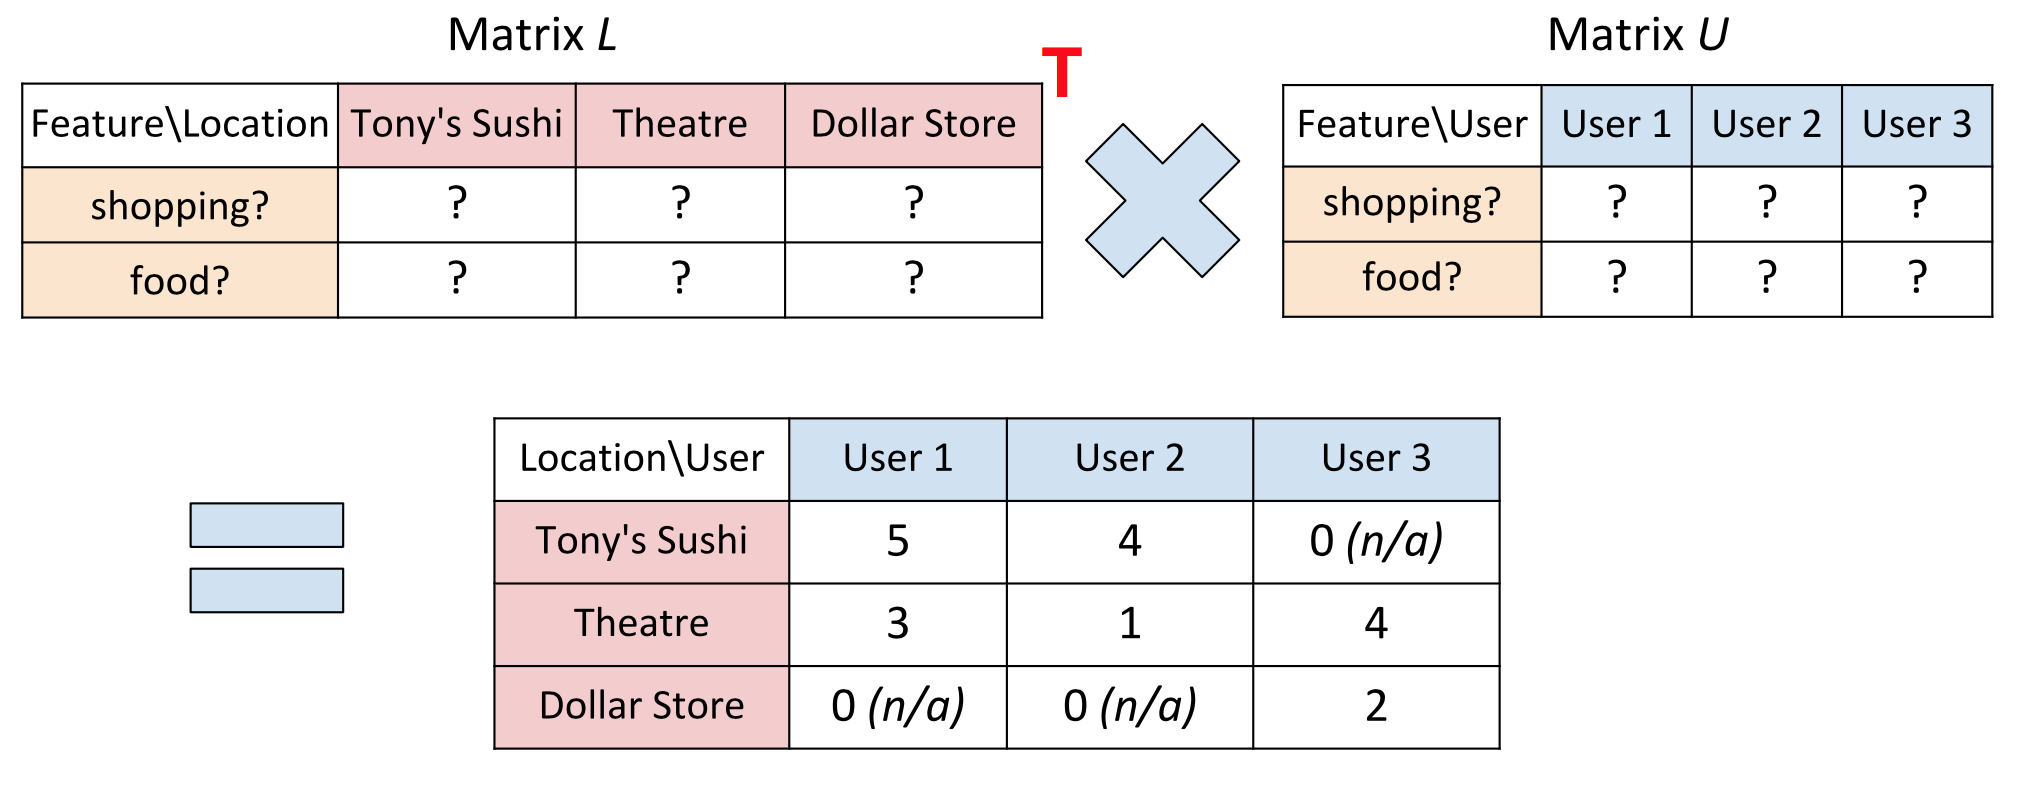
\psfig{file=MF.png,width=6in}
\caption{Matrix factorization of location-user matrix}
\label{fig:MF}
\end{figure*}

\begin{figure}
\centering
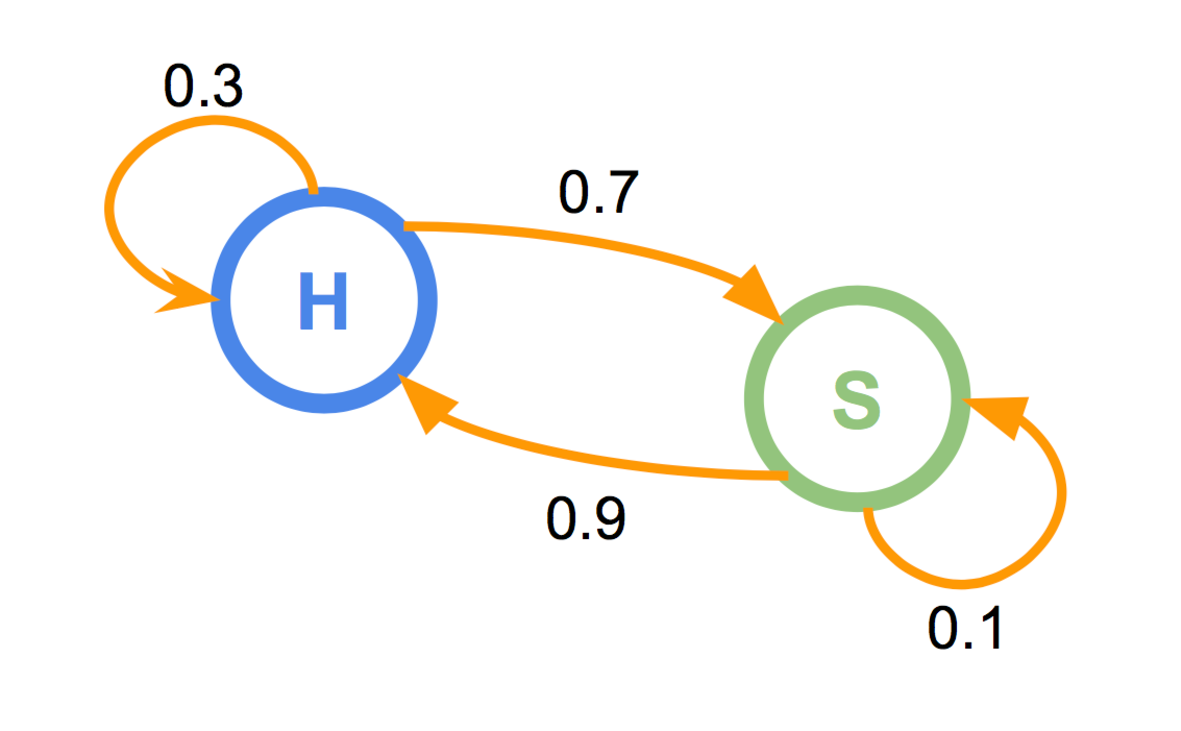
\psfig{file=MarkovChain.pdf,width=3in}
\caption{Markov chain with two states H (house) and S (school)}
\label{fig:MarkovChain}
\end{figure}

Traditionally, matrix factorization (MF) or Markov chain (MC) have been popular techniques for producing recommendations.
The ideas behind MF and MC will be explored in more detail in section \ref{sec:backgrounds}. 
Because of the known drawbacks of each model, Rendle et al. [2010] proposes factorizing personalized 
Markov chains (FPMC), which is the combination of MC and MF techniques. FPMC is a robust system, 
but it is a generic model and not designed for POI recommendations. To capture the locality feature of 
POI recommendations, Cheng et al. [2013] suggests FPMC-LR method where LR stands for localized regions. 
And, Li et al. [2017] proposes time-aware FPMC with time decaying consideration called TAD-FPMC.

In section 2, we are going to cover general and mathematical backgrounds in recommendation systems 
to understand the proposed models. Then in section 3, we will explore the proposed approaches in detail. 
In section 4, we will compare the accuracy of different recommendation techniques: FPMC, FPMC-LR, and TAD-FPMC. 
Finally, we will conclude the paper in section 5.



\section{Backgrounds}
\label{sec:backgrounds}


\textbf{Markov chain.} Markov chain (MC) is stochastic process widely adapted in many recommendation systems 
including movie, item, and POI recommendations. A MC is defined on a set of states; each state can be either a value
or a set of values. In the context of LBSN, each state represents a place where users can visit.
Now, we can define MC as a collection of transitional probabilities among different states.
In other words, it is a map of transitions from one state to another state. 

Figure \ref{fig:MarkovChain} shows a simple Markov chain 
model with two possible states: house (H) and school (S). The number labels on arrows represent 
the probability of the transition to the indicated direction. When the current state of the 
user is H, the probability of the user going to S (going to school) is 70\% and the probability of the 
user going to H (staying in the house) is 30\%. The diagram of states and transitions can also be 
represented as a transition probability matrix, which allows mathematical analysis. One important 
characteristic of the Markov chain is that predictions of future transitions are solely based on the present 
system. Therefore, the previous iterations and future iterations are completely independent. 
Just like the simply example above, we can easily imagine that Markov chain is directly applied to 
POI recommendation but with tens of thousands of places instead of two places. In practice, MC based 
approaches use one general transition matrix over all users. 

\textbf{Matrix factorizaion.} In Linear Algebra, matrix factorization (MF) is a technique to 
factor a matrix as a product of multiple matrices. When used in POI recommendation systems, 
the original matrix has two dimensions: locations and users. Each entry represents the rating of 
the place from the user. As you can see in Figure \ref{fig:MF}, the matrix
has many 0 entries which are the places users have never visited so no rating exists. 
Our goal is filling those empty entries by calculating predicted ratings. This is where MF takes on
a role. Using MF technique, the location-user matrix can be represented as a product of two matrices: 
a location matrix and a user matrix. As in Figure \ref{fig:MF}, both location matrix $L$ and user matrix $U$ share 
a latent factor space of dimensionality $f$. Each entry in $f$ is a feature that we can measure.
For instance, above matrices has two features: shopping? and food?. Once we find the two 
factors of A, we can make an estimation of unknown ratings. Let $q_l \in \mathbb{R}^f$ be a vector associated with location $l$, and 
$p_u \in \mathbb{R}^f$ be a vector associated with user $u$. The elements of $q_l$ show how related location $l$ is to its factors, 
and the elements of $p_u$ show how interested user $u$ is in the factors. If $r_{u,l}$ is the rating of location $l$ 
from user $u$, we can find the estimate as:
\begin{equation}
	r_{u,l}= q_l^T p_u
\label{eq:MF}
\end{equation}

The following are some clarifications on the estimation process:
\begin{itemize}
\item[--] The location-user matrix has many missing entries. Thus, the matrix factors ($U$ and $L$ from figure \ref{fig:MF}) are 
estimates whose product produces a matrix similar to the original matrix.
\item[--] The size of $f$ matters with respect to efficiency and accuracy. If $f$ is too small, we do not 
incorporate enough features for a precise recommendation. If $f$ is too large, it takes a very long time 
to compute the predictions. Hence, the number of features $f$ should be chosen carefully depending on 
the given circumstances.
\end{itemize}

\textbf{Tensor.} A tensor is essentially a quantity which can represented by a magnitude, a direction, and 
a dimension. Remember a vector is a quantity of a magnitude and a direction, and a scalar 
is a quantity of a magnitude. In fact, a vector is a tensor of rank 1 and a scalar is a tensor 
of rank 0. Simply put, a rank 2 tensor can be represented as a matrix, and higher rank tensors 
are thought as multi-dimensional version of the matrix. For instance, we can stack matrices on 
the top of one another to represent a 3 rank cube-shaped tensor. From Computer Science perspective, tensors can be 
thought as multi-dimensional arrays in programming languages.
Just like matrices, tensors can also be factorized. This is a key idea of many POI recommendation approaches 
that we will discuss more in next section.

\begin{figure*}
\centering
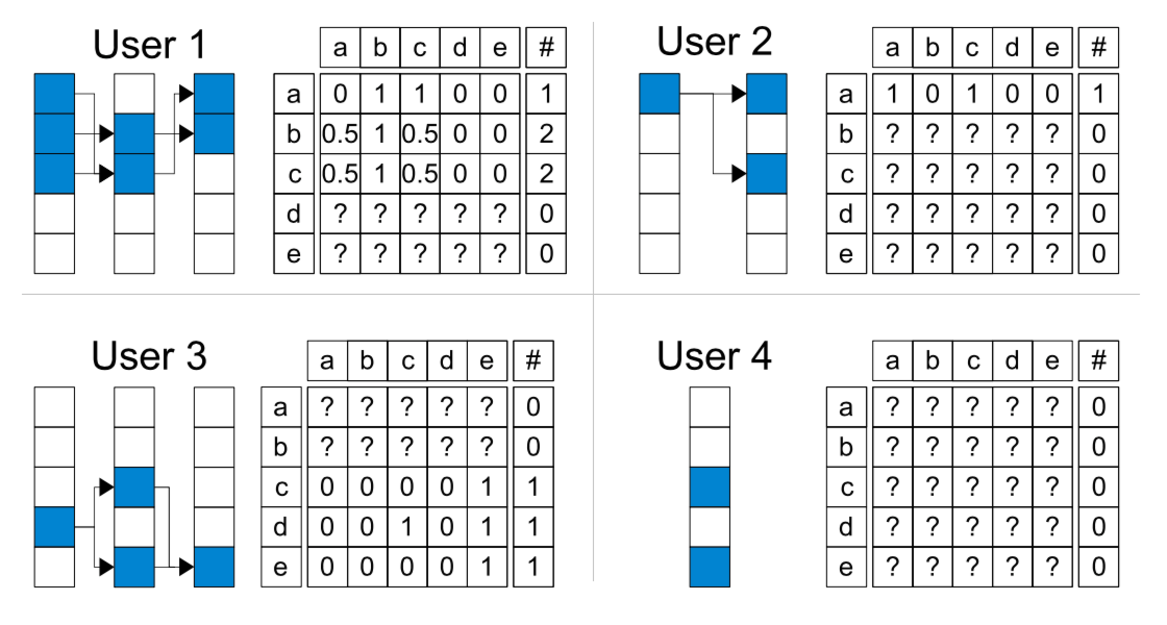
\psfig{file=FPMC_naive.pdf,width = 5in}
\caption{Personalized Markov chains.}
\label{fig:FPMC_naive}
\end{figure*}

\begin{figure}
\centering
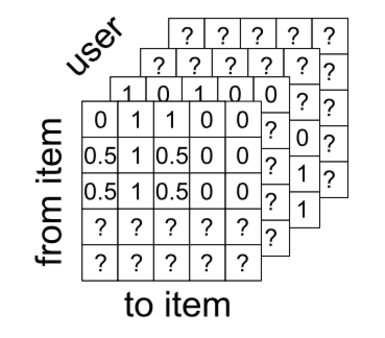
\psfig{file=FPMC.pdf,width= 2in}
\caption{Personalized transition tensor.}
\label{fig:FPMC}
\end{figure}

\section{Factoring Personalized Markov Chain and its improvements}
\label{sec:fpmc}

As we have discussed in section \ref{sec:backgrounds}, MC and MF based recommendation systems
have fairly distinct characteristics from each other. In this section, we will study a model called 
factorized personalized Markov chain (FPMC) that incorporates MF into MC, and its 
enhancements specializing in LSBN specific data properties.

\subsection{Formalization}
\label{sec:typeChangesSpecialChars}

Before we dive into the details of the algorithms, let us introduce the notation used in this paper. 
Let $U$ be a set of users and $L$ be a set of locations. For each user $u \in U$, 
we know their check-in history set \begin{math}L^t_u\end{math} where $t$ is the timestamp 
of a user visit. Our goal now is, given the user check-in data 
\begin{math}L^1_u,...,L^{t-1}_u\end{math}, recommend a next location to 
a user $u$ at time $t$. This goal is roughly equivalent to finding the probability of $u$ 
checking in location $l$ at time $t$, given a previous check-in location $i$ at time $t-1$:

\begin{equation}
	x_{u,i,l}=p(l \in L_u^t | i \in L_u^{t-1})
\label{eq:goal}
\end{equation}

\subsection{FPMC}
\label{sec:typeChangesSpecialChars}

Even though MC based recommendation systems were widely studied and used because of 
its capacity to capture sequential data, it lacks the personalization feature to distinguish each user. 
MF also has its weakness in processing sequential information since the order in a user's check-in sequence 
is often ignored when prediction is calculated.
In section \ref{sec:introduction}, we mentioned sequential information plays a huge role in LBSN 
in that there is a strong connection between users' recently visited locations and future locations. 
Imagine a POI recommendation system with no sequential awareness. 
It may recommend a family restaurant to a user who just check-ined a restaurant; this is not ideal. 
To take advantage of these two complementary models, Rendle et al. [2010] proposes FPMC.

First, let us think about what kind of recommendation model we aim to build. 
We want a recommendation system that is aware of sequential pattern and personalized for each user.
MC is good at recognizing sequential features, but it uses one general transition matrix for every user. 
Then, the question is, can we create a personalized MC?
A straightforward approach is having a personalized MC per user $u \in U$. 
Figure \ref{fig:FPMC_naive} shows four different transition matrices for each user. 
The question mark (?) entries mean we have no data to estimate the probability of the transition. The problem of these personalized 
MC matrices is that they are often very sparse, so they result in poor estimations. We just do not have enough data from
each user. This is the place where the ideas of MF can be applied. By stacking all transition matrices of users, 
we can get a transition cube or tensor $\chi$. Now, we can factorize the tensor using a tensor factorization technique. 
Factorizing this tensor $\chi$ produces four parameters: one rank-3 core tensor and three groups of matrices. Using an efficient tensor 
factorization technique pairwise interaction tensor factorization (PITF), we get the following 
estimation equation for the probability of user $u$ going to location $l$ from location $i$:

\begin{equation}
	\hat{x}_{u,i,l} := v_u^{U,L} \cdot v_l^{L,U} + v_l^{L,I} \cdot v_i^{I,L} + v_u^{U,I} \cdot v_i^{I,U}
\label{eq:MF}
\end{equation}

This is the essence of FPMC method. To achieve the recommendation goal $\hat{x}_{u,i,l}$, we 
construct a tensor containing MCs for users, and then we factorize the tensor into a rank-3 tensor 
and matrices. Finally, we calculate the prediction by combining the corresponding entries of the
factors. 

\subsection{FPMC-LR}
\label{sec:typeChangesSpecialChars}

FPMC successfully constructs a personalized MC for POI recommendation
by combining ideas of MF and MC. However, it overlooks another noticeable property 
of LBSN dataset, localized region constraint. According to check-in data from 
Gowalla and Foursquare, more than 75\% of check-ins from Foursquare and 80\% of check-ins 
from Gowalla happened within 10 km of the previously checked-in place. The observation on the LBSN data
shows the trend that users tend to check in places close to their previous check-ins, 
but FPMC does not really make use of this potentially useful trend.

To add the ability to use localized region constraint 
information into the existing FPMC model, Cheng et al. [2013] 
introduces a model called FPMC-LR which combines FPMC model with localized 
region (LR) constraints to provide accurate successive POI recommendation in LBSNs. 
Because FPMC-LR only takes into account nearby candidate locations depending 
on where the users currently are, it reduces the computational costs and noisy information. 
Also, it results in more accurate predictions as we will see in section \ref{sec:experiments}.

FPMC-LR model has a similar setting to FPMC since it is an improvement 
over FPMC. Just like FPMC, the fundamental goal of FPMC-LR is to give the most suitable 
location recommendation for user $u$ at time $t$, given a sequence of check-in data. 
In other words, we need to calculate $x_{u,i,l}$, which is the probability of a user $u$ to visit a location $l$ at time $t$,
where $i$ is the user location at time $t-1$.
The main difference between FPMC and FPMC-LR is in their transition tensor. As we saw earlier, FPMC takes into account 
all possible locations for each user, so the tensor looks like: 
\begin{equation}
	\chi \in [0, 1]^{|U| \times |L| \times |L|}
\label{eq:summation}
\end{equation}
On the other hand, FPMC-LR only considers neighborhood locations of the previous check-in location $i$. 
The tensor transition in FPMC-LR looks like:
\begin{equation}
	\chi \in [0, 1]^{|U| \times |L| \times |N_d(L)|}
\label{eq:summation}
\end{equation}
The set of neighborhood locations \begin{math}N_d(L)\end{math} is calculated by Haversine formula, 
which is used to find the shortest distance between two points on the surface of a sphere. 
In this case, we assume the earth is roughly a sphere. By applying the same tensor factorizing technique to 
our tensor $\chi \in [0, 1]^{|U| \times |L| \times |N_d(L)|}$, we get the target probability $x_{u,i,l}$.

\subsection{TAD-FPMC}
\label{sec:typeChangesSpecialChars}

FPMC-LR is a very successful model for POI recommendation in terms of performance and efficiency 
as we will discuss in later section; it incorporates sequential data with personalization and locality consideration. 
However, there is a still room for improvement. Li et al. [2017] points out that FPMC-LR approach simply captures 
the consecutive ordering relations in lieu of considering complex user behavior over time. Take college students, 
for example. Students have morning classes, afternoon classes, or both in one day. When they have morning classes, 
some of them have breakfast at a brunch cafe after class. When they have afternoon classes, some of them go 
for a drink at a bar after class. Simply combining them as one sequential pattern is clearly not sufficient (e.x. recommending 
for a drink at a bar after 8:00AM class). In other words, just recognizing sequential data is not 
enough for capturing the differences in regular periodic pattern.

To make the system consider users' time-varying behavioral trends, Li et al. [2017] suggests time-aware FPMC (TA-FPMC) 
model, which is an improvement over FPMC-LR model. In section 2-1, Rendle et al. [2010] uses third order tensor to 
construct a personalized Markov chain. TA-FPMC takes a similar approach. Instead of a third order tensor of 
user-location-location, it forms a fourth order tensor by adding a time factor. Now, the transition tensor looks like: 
\begin{equation}
	\chi \in [0, 1]^{|U| \times |T| \times |L| \times |L|}
\label{eq:TA-FPMC_tensor}
\end{equation}
There is another statistical characteristic of LBSN data that has not got much attention, the time gap between 
two successive check-ins. The LBSN data shows that many of two successive check-ins span a large time gap 
like a year. Base on the assumption that these successive check-ins with large time gaps do not tell much, 
Li et al. [2017] introduces another factor $D(\Delta t)$ to take into account the time-decaying effect. 
The final model with all the considerations is called TAD-FPMC.

\section{Experiments}
\label{sec:experiments}
In the experiments, we will address the following questions: 1) How do different POI recommendation 
models perform in real LBSN data? 2) Why are distance constraint and temporal information particularly important 
factors in POI recommendation?

\subsection{Datasets}
\label{sec:datasets}
The evaluation used data collected from Foursquare, a LBSN that provides POI recommendations based on 
each user's preference. The data includes users' check-in data of New York City and Los Angeles from Jan. 
2010 to June 2011. Li et al. [2017] divided available locations in the data into 249 categories. 
The summary of the statistics is elaborated in Table 1. In Table 1, \emph{tip} means comments or reviews on a 
certain location written by other users.

\subsection{Evaluation Metric}
\label{metic}
The main task for models is providing a list of top-N locations (the list contains N locations 
ordered from the highest probability of user visit to the lowest). The recommendation is considered 
correct if the user indeed visited a location in the top-N list or the category of the user visit location 
is in the top-N list. The evaluation metric is defined as:
\begin{equation}
	P@N = \frac{\textrm{the counts of correct predictions}} {\textrm{the total number of recommendation rounds}}
\label{eq:P@N}
\end{equation}


\subsection{Comparison}
\label{comparison}
Figure * shows the performance comparison among different models of POI recommendation. 
The x-axis represents the N value which is the number of recommended locations, and the y-axis 
is the precision of the recommendation P@N. In both LA and NYC data, there is a huge gap 
between generic models (MF and FPMC) and POI specific models (FPMC-LR and TAD-FPMC). 
This verifies the importance of distance constraint and temporal information in POI recommendations. 
Also, TAD-FPMC slightly outperforms FPMC-LR in both datasets. If we utilize additional enhancements 
for TAD-FPMC, the performance improves significantly as we can see in Table .

The experiments were run on a machine with a Core i7-6700K 4.0GHz 8HT and memory size of 32GB. 
In terms of the efficiency, TAD-FPMC is shown to be the most efficient model with the running time of 
3 hours compared to FPMC and FPMC-LR with 35 hours. The reduced dimensionality from the number of 
locations to the number dimensionality improves the efficiency significantly.

\section{Conclusions}
\label{sec:conclusions}

In this paper, we have considered the task of point-of-interest (POI) recommendation in LBSNs 
and introduced different approaches for accurate predictions. Factorized personalized Markov 
chain (FPMC) model is an elegant method combining advantages of Markov chains and matrix factorization,
but it was not designed to incorporate distinct characteristics of LBSN data. FPMC-LR is an enhancement 
of FPMC by only considering nearby locations when calculating POI predictions. TAD-FPMC is a novel 
POI recommendation system approach that captures complex user behavior over time in addition to inheriting strengths 
of FPMC and FPMC-LR models. From experimental results conducted on Foursquare data, we conclude 
POI recommendation specific approaches (FPMC-LR, TAD-FPMC) far outperform generic recommendation models such as FPMC.
Additionally, TAD-FPMC produces better predictions than any other methods including FPMC-LR.


\section*{Acknowledgments}
\label{sec:acknowledgments}

This section is optional; it is a location for you
to acknowledge grants, funding, editing assistance and
what have you.

You want to use the \texttt{\textbackslash section*} version of the \texttt{section}
command, as an acknowledgments section typically does \emph{not} get
a number.

It is common (but by no means necessary) for students to thank
their advisor, and possibly other faculty, friends, and family who provided
useful feedback on the paper as it was being written.

In the present case, for example, the
authors would like to thank Gerald Murray of ACM for
his help in codifying this \textit{Author's Guide}
and the \textbf{.cls} and \textbf{.tex} files that it describes.

% The following two commands are all you need in the
% initial runs of your .tex file to
% produce the bibliography for the citations in your paper.
\bibliographystyle{abbrv}
% sample_paper.bib is the name of the BibTex file containing the
% bibliography entries. Note that you *don't* include the .bib ending here.
\bibliography{sample_paper}  
% You must have a proper ".bib" file
%  and remember to run:
% latex bibtex latex latex
% to resolve all references

\end{document}
